\chapter{Human Preference Score Metric}
\label{ch:hpsv3}

% \item \acs{VLM} (Vision Language Model) metric and filtering method. Implement the HPSv3 VLM metric (a model trained to emulate a human preference score) to evaluate the model's performance on individual images which helps on a couple of fronts:
%     \begin{itemize}
%         \item the FID metric is a good simple metric to start with in the field of natural images generation but it has been criticized in the literature \parencite{jayasumana_rethinking_2024} to contradict humans. Precision and Recall are built on the same feature extractor as the FID and are therefore also affected by this criticism leading to the need for an alternative for the \acs{FPR} set of metrics.
%         \item the \acs{FPR} metrics can only be computed on batches of generated samples. Testing the metric on small batches is brittle and creating big batches of images is very expensive. 
%         % \item Avoiding the task of manually reviewing the images and their score to make sure the uncertainty scoring method is properly.
%     \end{itemize}

\cite{jazbec_generative_2025} has relied on the \acs{FPR} (FID, Precision and Recall) metrics to evaluate the performance of generative uncertainty against other baselines such as Realism, Rarity and BayesDiff \parencite{kou_bayesdiff_2024}.
While the \acs{FPR} metrics are a good starting point in the field of natural images, we provide an extensive list of its problems in \autoref{sub:problems_inception}. Those problems motivated the need for a new independent metric that align better with human preferences and can be computed on single images at a time.


% \cite{jayasumana_rethinking_2024} proposed using an alternative feature extractor to improve the FID metric. But to satisfy our additional need for a \textit{per-image} metric, we went with a model trained to predict Human Preference Scores per image.

% Those metrics are standard in the field of diffusion models but may not be the most accurate at judging if we are effectively removing hallucinations.

% One issue of \parencite{jazbec_generative_2025} framework was that FID, precision, recall, realism and rarity all work in the same \textit{inception-net} feature space which offers a biased evaluation of the realism and rarity baselines against generative uncertainty.

\section{Human Preference Score v3 (HPSv3)}

If the idea of generative uncertainty on natural images is to detect hallucinations, supposing that humans are good judges at flagging hallucinations as bad images (lower scores) and normal looking images as high scores, an \acs{HPS} should align well with generative uncertainty.
It should be noted however that part of the human score is also attributed to how pleasant it is to look at the image, which is not what hallucinations are about, we therefore do not expect a perfect correlation.

For this experiment, we went with the HPSv3 score \parencite{ma_hpsv3_2025}, it supports both high quality and low quality pictures which is essential for our low quality 128x128 ADM model.

The HPSv3 score however is built to judge how much a text description matches an image. The \acs{ADM} model on the other hand is built to generate class conditioned images such as dog, flower,... To make the HPSv3 score work with this setup we just use the following text description for each image: ``\texttt{a high quality photo of a [class\_name]}''

% We can immediately compute the correlation score of 

\section{Measuring HPSv3 Performance on FID, Precision, Recall}

We can first use HPSv3 as a filtering metric and compare it to the other usual baseline (Realism, Rarity, \acs{GU}) on the \acs{FPR} metrics.

\begin{figure}[!htbp]
    \centering
    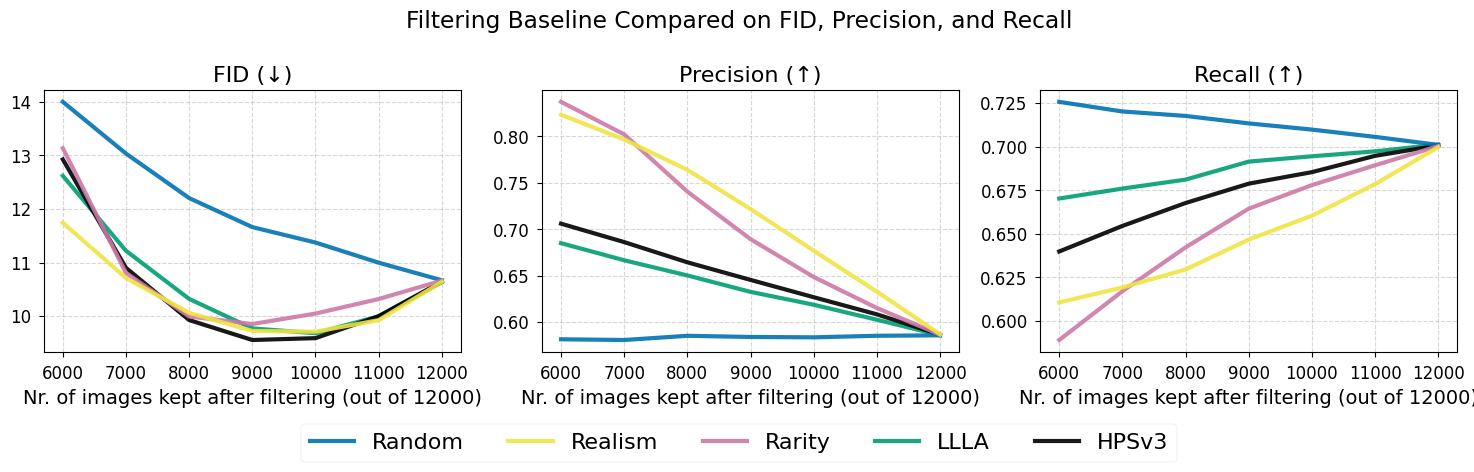
\includegraphics[width=0.9\linewidth]{figures/hps/fpr.png}
    \caption{Comparison of performance of different filtering methods on FID, Precision, Recall. \warning, we are using new colors here}
    \label{fig:hps_fpr}
\end{figure}

We can see on \autoref{fig:hps_fpr} that HPSv3 actually outperforms Generative Uncertainty \acs{GU} (LLLA) on FID and Precision at the cost of a lower Recall. This can at least motivate that the HPSv3 metric is compatible with what \cite{jazbec_generative_2025} \acs{GU} tries to measure and since it seem to mostly outperform \acs{GU}, it can serve as a standalone metric, oracle to say judge how well a filtering metric is improving the ``true'' visual quality of the dataset as perceived by humans.

\section{Using HPSv3 as a Standalone Evaluation Metric}

We can now try to use HPSv3 as a standalone evaluation metric to compare the different filtering baselines.

We first define the error $\mathcal{E}$ as
\begin{equation}
\mathcal{E}(i) = \max_{j \in {D_{gen}}}(\mathrm{hpsv3}(j)) - \mathrm{hpsv3}(i)
% \text{avg error} = \sum_{i \in \{j | m(j) <\}} (\max(\mathrm{hpsv3}_{i}) - \mathrm{hpsv3}_{i})
\end{equation}
With $D_{gen}$ being the dataset of generated samples (images) and $i,j$ being samples drawn from $D_{gen}$.
The bigger the error $\mathcal{E}$ of a sample, the lower it's hpsv3 score.

\begin{tcolorbox}[colback=orange!10!white,colframe=orange!50!black,sharp corners]
It was later observed that using the maximum value of the hpsv3 metric across a single generated dataset as anchor point for the error metric is very unstable across different generated datasets (obtained instance by changing the random seed). In this thesis we never compare hpsv3 metrics results across different generated datasets.
\end{tcolorbox}

We are once again using a rejection rate $r$ which is the percentage of images (performing the worse on a metric) that we filter out.
To measure how well the filtering works with respect to hpsv3, we compute the average error $\overline{\mathcal{E}}$ across the remaining samples at each $r$ during the filtering.

Additionally, to summarize the rejection curve with a single number, we define the \acs{AURC} (Area Under the Rejection Curve):
\begin{equation}
\mathrm{AURC}=\int_0^{1}\overline{\mathcal{E}}(r)dr
\end{equation}

\begin{figure}[!htbp]
    \centering
    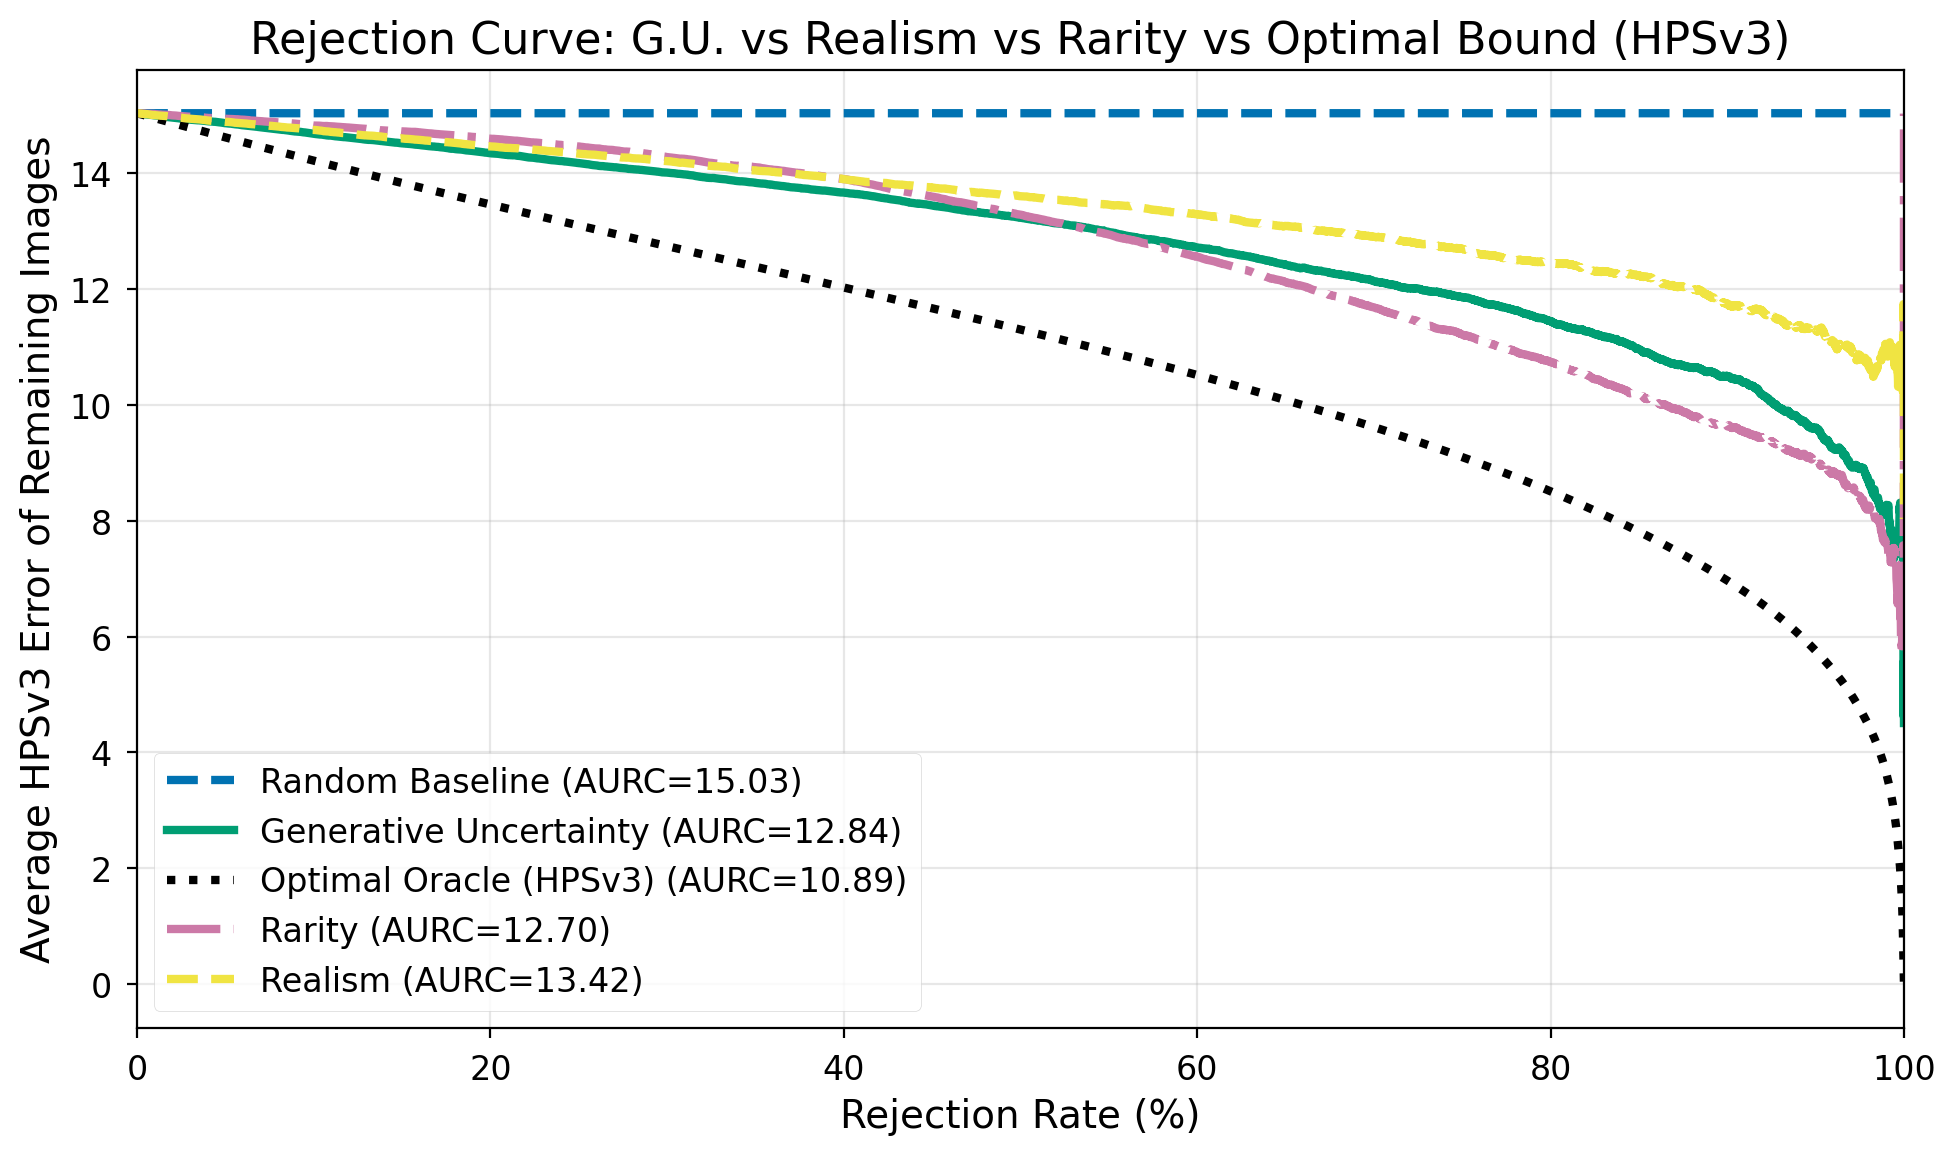
\includegraphics[width=0.9\linewidth]{figures/hps/rejection_curve.png}
    \caption{Comparison of how close \acs{GU}, Realism, Recall manage to get to HPSv3.}
    \label{fig:hps_rejection_curve}
\end{figure}

As we can see on \autoref{fig:hps_rejection_curve}, \acs{GU} performs best at first and later gets outperformed by Rarity. 
% It is worth noting however that most images generated from ADM being of low perceptual, we should be less interested of what happens at higher rejection rates.

\section{Conclusion}
\texttt{HPSv3} proved to be a capable filtering metric, motivating its use as an evaluation metric on top of the \acs{FPR} set of metrics to have an additional judgment of the filtering baselines that does not have the flaws from \acs{FPR} (\autoref{sub:problems_inception}). 